\documentclass[12pt, twoside]{article}
\documentclass[12pt, twoside]{article}
\usepackage[letterpaper, margin=1in, headsep=0.2in]{geometry}
\setlength{\headheight}{0.6in}
%\usepackage[english]{babel}
\usepackage[utf8]{inputenc}
\usepackage{microtype}
\usepackage{amsmath}
\usepackage{amssymb}
%\usepackage{amsfonts}
\usepackage{siunitx} %units in math. eg 20\milli\meter
\usepackage{yhmath} % for arcs, overparenth command
\usepackage{tikz} %graphics
\usetikzlibrary{quotes, angles}
\usepackage{graphicx} %consider setting \graphicspath{{images/}}
\usepackage{parskip} %no paragraph indent
\usepackage{enumitem}
\usepackage{multicol}
\usepackage{venndiagram}

\usepackage{fancyhdr}
\pagestyle{fancy}
\fancyhf{}
\renewcommand{\headrulewidth}{0pt} % disable the underline of the header
\raggedbottom
\hfuzz=2mm %suppresses overfull box warnings

\usepackage{hyperref}

\fancyhead[LE]{\thepage}
\fancyhead[RO]{\thepage \\ Name: \hspace{4cm} \,\\}
\fancyhead[LO]{BECA / Dr. Huson / Geometry\\*  Unit 9: Similarity and proportions \\* 5 April 2023}

\begin{document}

\subsubsection*{9.11 Test: Dilation, transformations, and similarity}
I can solve problems using similarity criteria. \hfill CCSS.HSG.SRT.B.5
\begin{enumerate}
\item Dilate $\triangle ABC \rightarrow \triangle A'B'C'$ by a factor of $k=3$ centered at the origin, \\
$(x,y) \rightarrow (3x, 3y)$. Plot and label the image on the axes.
\begin{center}
    \begin{tikzpicture}[scale=1]
    \draw [help lines] (-1,-2) grid (8,8);
    \draw [thick, <->] (-1.4,0) -- (8.4,0) node [right] {$x$};
    \draw [thick, <->] (0,-2.4)--(0,8.4) node [above] {$y$};  
    \draw [thick]
        (0,0) node[below left] {$A$}--
        (2,2) node[above left] {$B$}--
        (2, 0) node[below left] {$C$}--cycle;  
    \end{tikzpicture}
\end{center}

\item A dilation centered at $A$ with scale factor $k=2$ maps $\triangle ABC \rightarrow \triangle ADE$. Given the lengths $AC = 10$, $BC = 7$, $AB = 12$, and $DE = 14$. \\[0.25cm]
How long are $AD$ and $AE$?
    \begin{flushright}
    \begin{tikzpicture}[scale=0.8]
        \draw [-, thick] (0,0)--
        (8,0) node[below]{$E$}--
        (8,6) node[right]{$D$}--cycle;
        \draw [thick] (4,0)--(4,3);
        \draw [fill] (0,0) circle [radius=0.1] node[below] {$A$};
        \node at (4,0) [below]{$C$};
        \node at (4,3) [above left]{$B$};
        \node at (2, 0) [below]{$10$};
        \node at (2, 2) [above]{$12$};
        \node at (8, 3) [right]{$14$};
        \node at (4, 1.5) [right]{$7$};
    \end{tikzpicture}
    \end{flushright}

\newpage
\item Given $\triangle ABC \sim \triangle DEF$, $m\angle A=35^\circ$, and $m\angle F=105^\circ$. Find $m\angle C$. \vspace{4cm}

\item What is the transformation mapping parallelogram $BECA \rightarrow B'E'C'A'$, as shown in the diagram. (hint: Dilations must specify the center and scale factor.)
    \begin{flushright}
        \begin{tikzpicture}[scale=1]
        \draw [help lines] (-1,-1) grid (7,6);
        \draw [thick, <->] (-1.4,0) -- (7.4,0) node [right] {$x$};
        \draw [thick, <->] (0,-1.4)--(0,6.4) node [above] {$y$};  
        \draw [thick]
            (0,0) node[below left] {$B$}--
            (1,2) node[above left] {$E$}--
            (3,2) node[above right] {$C$}--
            (2,0) node[below right] {$A$}--cycle;
        \draw [thick]
            (0,0) node[below right] {$B'$}--
            (2,4) node[above left] {$E'$}--
            (6,4) node[above right] {$C'$}--
            (4,0) node[below right] {$A'$}--cycle;
        \end{tikzpicture}
    \end{flushright}

\item A dilation maps $\triangle ABC \rightarrow \triangle ADE$. Given $AB=9$, $AC=11.1$, $BC=6$, $DE=14$. 
\begin{multicols}{2}
    Find the scale factor and side lengths:\\[0.5cm]
    $k=$\\[1cm]
    $AD=$\\[1cm]
    $AE=$\\[1cm]
    $BD=$\\
    \begin{flushright}
    \begin{tikzpicture}[scale=1.]
        \draw [thick]
        (0,0)node[below]{$A$}--
        (0:6)node[below]{$D$}--
        (30:8)node[above]{$E$}--cycle;
        \draw [thick]
        (0:2.4)node[below]{$B$}--
        (30:3.2)node[above left]{$C$};
        \node at (0:1.5)[below]{$9.0$};
        \node at (15:2.7)[right]{$6.0$};
        \node at (15:6.75)[right]{$14.0$};
        \node at (35:1.7)[above]{$11.1$};
    \end{tikzpicture}
    \end{flushright}
\end{multicols}\vspace{0.25cm}

\newpage
\item Steven and Marie live close to school and Tio's bodega, but also like to go to Grandma's house and the baseball field, which are further away. A sketch of the locations is shown below, essentially two triangles with a scale factor $k=2$ centered at home.\\[0.25cm]
From home it's 3 blocks to school and 4 to the bodega. From Grandma's to the baseball field is 10 blocks. There are twenty blocks to a mile.
\begin{enumerate}
    \item Steven stops at the bodega before continuing on his way to school. How far does he walk on this way to school, in terms of both blocks and miles?
        \begin{flushright}
            \begin{tikzpicture}[scale=0.6, rotate=-13]
            \draw [thick]
            (0,0)node[above]{$Home$}--
            (-130:10)node[below]{$Baseball$}--
            (-40:7.5)node[below]{$Grandma's$}--cycle;
            \draw [thick]
            (-130:5)node[above left]{$Bodega$}--
            (-40:3.75)node[right]{$School$};
            \node at (-155:2.5)[below]{$4$};
            \node at (-35:1.5)[right]{$3$};
            \node at (-95:7.5)[above]{$10$};
            \end{tikzpicture}
        \end{flushright} 
    \item Marie plays baseball after school. Which route from school to baseball is shorter, passing by the bodega or the way by Grandma's? By how many blocks is it shorter? Justify your answer.
\end{enumerate} \vspace{4cm}

\item Given $\triangle ABP \sim \triangle JKP$ as shown below. $AB=10$, $AP=9.0$, $PK=12.5$, and $JK=25$. Find $JP$ and $BP$.
  \begin{flushright}
  \begin{tikzpicture}[scale=1.6]
      \draw [thick]
        (-0.25,-1)node[below left]{$B$}--
        (0.5,2)node[left]{$K$}--
        (4,0)node[below left]{$J$}--
        (0,0)node[above left]{$P$}--
        (-2,0)node[left]{$A$}--cycle;
    \end{tikzpicture}
    \end{flushright}

\newpage
\item The vertices of $\triangle JKL$ have the coordinates $J(0,-1)$, $K(5,2)$, and $L(1,4)$, as shown.
\begin{enumerate}
    \item Apply a dilation to $\triangle JKL \rightarrow \triangle J'K'L'$, centered at $P(2,2)$ and with a scale factor $k=2$. Draw the image $\triangle J'K'L'$ on the set of axes below, labeling the vertices.
        \begin{center}
        \begin{tikzpicture}[scale=.48]
            \draw [help lines] (-9,-8) grid (9,8);
            \draw [thick, <->] (-9.4,0) -- (9.4,0) node [right] {$x$};
            \draw [thick, <->] (0,-8.4)--(0,8.4) node [above] {$y$};
            \draw [thick]
            (0,-1) node[below right] {$J$}--
            (5,2) node[below right] {$K$}--
            (1,4) node[above right] {$L$}--
            cycle;
            \fill (2,2) circle[radius=0.15cm]node[below right]{$P$};
        \end{tikzpicture}
        \end{center}
    \item What is the ratio of the area of $\triangle JKL$ to $\triangle J'K'L'$?
    \end{enumerate} \vspace{2cm}

\item Triangle $ADE$ is drawn with $\overline{BC} \parallel \overline{DE}$, as shown. Given $AB=5$, $BC=8$, $AC=8$, and $BD=5$. $m\angle A = 72^\circ$. \\[0.25cm] 
Find m$\angle ABC$ and m$\angle E$.
%Find $CE$, $AE$, and $DE$. Find and mark all of the angle measures of the triangle.\vspace{1cm}
    \begin{flushright}
        \begin{tikzpicture}[scale=0.6]
        \draw [thick]
        (0.5,1.5)node[left]{$B$}--
        (6.5,1.5)node[above right]{$C$}--
        (2,6)node[above]{$A$}--cycle;
        \draw [thick]
        (0.5,1.5)--
        (-1,-3)node[left]{$D$}--
        (11,-3)node[above right]{$E$}--(6.5,1.5);
        \node at (3,1.5)[below]{$8$};
        \node at (4.5, 4)[right]{$8$};
        \node at (0.6, 3.3)[above]{$5$};
        \node at (-0.7, -1)[above]{$5$};
        \end{tikzpicture}
    \end{flushright}

\newpage
\item The line $\overleftrightarrow{AB}$ has the equation $y=\frac{1}{2}x-2$. Apply a dilation mapping $\overleftrightarrow{AB} \rightarrow \overleftrightarrow{A'B'}$ with a factor of $k=2.5$ centered at the origin. Draw and label the image on the grid. Write the equation of the line $\overleftrightarrow{A'B'}$.
  \begin{flushright}
  \begin{tikzpicture}[scale=.635]
    \draw [help lines] (-1,-7) grid (10,1);
    \draw [thick, ->] (-1.2,0) -- (10.4,0) node [below right] {$x$};
    \draw [thick, ->] (0,-7.2)--(0,1.4) node [left] {$y$};
    \draw [<->, thick] (-0.5,-2.25)--(4.5,0.25);
    \draw [fill] (0,-2) circle [radius=0.1]node[above left]{$A$};
    \draw [fill] (4,0) circle [radius=0.1]node[above left]{$B$};
  \end{tikzpicture}
  \end{flushright} \vspace{1cm}

\item Triangle $ADE$ and its midline $\overline{BC}$ are drawn, with $B$ the midpoint of $\overline{AD}$ and $C$ the midpoint of $\overline{AE}$. The two medians $\overline{BE}$ and $\overline{CD}$ are drawn, as shown, intersecting in point $F$, the centroid. Given $BC=10$, $FE=15$.
\begin{multicols}{2}
\begin{enumerate}[itemsep=1.5cm]
    \item Write down $DE$.
    \item Given $\triangle FCB \sim \triangle FDE$ with scale factor $k=2$. \\[0.25cm]
    Find $BF$.
    \item Given the area of $\triangle ABC$ is 50, find the area of $\triangle ADE$.
\end{enumerate}
\begin{center}
    \begin{tikzpicture}[scale=0.55]
    \draw [thick]
    (0.5,1.5)node[left]{$B$}--
    (6.5,1.5)node[above right]{$C$}--
    (2,6)node[above]{$A$}--cycle;
    \draw [thick]
    (0.5,1.5)--
    (-1,-3)node[below]{$D$}--
    (11,-3)node[below]{$E$}--(6.5,1.5);
    \draw [thick] (0.5,1.5)--(11,-3);
    \draw [thick] (6.5,1.5)--(-1,-3);
    \node at (3,2.5)[below]{$10$};
    \node at (3.5, -0.6)[right]{$F$};
    \node at (6.6, -.9)[above]{$15$};
    \end{tikzpicture}
\end{center}
\end{multicols}


\newpage
\item In the diagram below, the chords $\overline{AE}$ and $\overline{BD}$ intersect at $C$, with $\triangle ABC \sim \triangle DEC$, $BC=4$, $AC=5$, and $BD=11.5$. Determine the length of $\overline{CE}$.
    \begin{center}
    \begin{tikzpicture}[scale=.6]
    \draw (0,0) circle[radius=5];
    \draw [thick]
    (20:5) node[right] {$A$}--
    (160:5) node[left] {$E$}--
    (210:5) node[left] {$D$}--
    (50:5) node[above right] {$B$}--cycle;
    \draw (75:1.8) node[above] {$C$};
    \end{tikzpicture}
\end{center} \vspace{2cm}

\item In the diagram below $\triangle ABC \sim \triangle DEF$, $DE=x+4$, $AB=12$, $AC=21$, $DF=2x+4$. \\[0.25cm] 
Solve for $x$.
\begin{center}
    \begin{tikzpicture}[scale=1]
    \coordinate [label=above left:$A$](A) at (85:2);
    \coordinate [label=below:$B$](B) at (0, 0);
    \coordinate [label=right:$C$](C) at (-20:3);
    \draw [thick] (A)--(B)--(C)--cycle;
    \node at (95:1)[left]{$12$};
    \node at (35:1.75)[right]{$21$};
    \draw [thick, xshift=5cm, yshift=0.5cm] (85:3) node[above]{$D$}--
    (0,0) node[below]{$E$}--
    (-20:4.5) node[right]{$F$}--cycle;
    \draw [thick, xshift=5cm, yshift=0.5cm](90:1.5) node[left]{$x+4$};
    \draw [thick, xshift=5cm, yshift=0.5cm](30:2.75) node[right]{$2x+4$};
\end{tikzpicture}
\end{center}
  
\newpage
\subsubsection*{Extra}

\item Given $\triangle ABP \sim \triangle JKP$. $AB=7$, $AP=6.3$, $KP=8.8$, $JK=16.0$, $m\angle A=25^\circ$, $m\angle JPK = 105^\circ$. Solve the triangles (all angles and lengths).
\begin{flushright}
    \begin{tikzpicture}[scale=1.6]
        \draw [thick]
        (0.25,-1)node[right]{$B$}--
        (-0.5,2)node[left]{$K$}--
        (4,0)node[right]{$J$}--
        (0,0)node[above right]{$P$}--
        (-2,0)node[left]{$A$}--cycle;
    \end{tikzpicture}
\end{flushright} \vspace{2cm}

\item Dilate $\triangle ABC \rightarrow \triangle A'B'C'$ by a factor of $k=3$ centered at the origin, $(x,y) \rightarrow (3x, 3y)$. Plot and label the image on the axes. %Make a table of the vertices and their coordinates.
    \begin{flushright}
        \begin{tikzpicture}[scale=1]
        \draw [help lines] (-1,-3) grid (7,7);
        \draw [thick, <->] (-1.4,0) -- (7.4,0) node [right] {$x$};
        \draw [thick, <->] (0,-3.4)--(0,7.4) node [above] {$y$};  
        \draw [thick]
            (0,0) node[below left] {$A$}--
            (2,1) node[above left] {$B$}--
            (1,-1) node[below left] {$C$}--cycle;  
        \end{tikzpicture}
    \end{flushright}

\item Dilate $\triangle ABC \rightarrow \triangle A'B'C'$ by a factor of $k=1.5$ centered at the origin,\\
$(x,y) \rightarrow (1.5x, 1.5y)$. Plot and label the image on the axes. Make a table of the vertices and their coordinates.
\begin{flushright}
    \begin{tikzpicture}[scale=0.8]
    \draw [help lines] (-1,-2) grid (9,9);
    \draw [thick, <->] (-1.4,0) -- (9.4,0) node [right] {$x$};
    \draw [thick, <->] (0,-2.4)--(0,9.4) node [above] {$y$};  
    \draw [thick]
        (0,0) node[below left] {$A$}--
        (2,4) node[above left] {$B$}--
        (4,0) node[below] {$C$}--cycle;  
    \end{tikzpicture}
\end{flushright}

\item A transformation is performed on a parallelogram, $MATH \rightarrow M'A'T'H'$, as shown in the diagram. \\[0.5cm]
What is the transformation? (Hint: Is it a translation, reflection, rotation, or dilation? What is its center? What is the scale factor, $k$?)
\begin{flushright}
    \begin{tikzpicture}[scale=0.7]
    \draw [help lines] (-1,-3) grid (10,7);
    \draw [thick, <->] (-1.4,0) -- (10.4,0) node [right] {$x$};
    \draw [thick, <->] (0,-3.4)--(0,7.4) node [above] {$y$};  
    \draw [thick]
        (0,0) node[below left] {$M$}--
        (1,2) node[above left] {$A$}--
        (3,2) node[above left] {$T$}--
        (2,0) node[below right] {$H$}--cycle;
    \draw [thick]
        (0,0) node[below right] {$M'$}--
        (3,6) node[above right] {$A'$}--
        (9,6) node[above right] {$T'$}--
        (6,0) node[below right] {$H'$}--cycle;
    \end{tikzpicture}
\end{flushright}

\item Dilate $\triangle ABC \rightarrow \triangle A'B'C'$ by a factor of $k=1.5$ centered at the origin, $(x,y) \rightarrow (1.5x, 1.5y)$. Plot and label the image on the axes. Make a table of the vertices and their coordinates.
    \begin{flushright}
    \begin{tikzpicture}[scale=1]
    \draw [help lines] (-1,-2) grid (5,7);
    \draw [thick, <->] (-1.4,0) -- (5.4,0) node [right] {$x$};
    \draw [thick, <->] (0,-2.4)--(0,7.4) node [above] {$y$};  
    \draw [thick]
        (0,0) node[below left] {$A$}--
        (2,4) node[above left] {$B$}--
        (2,0) node[below] {$C$}--cycle;  
    \end{tikzpicture}
    \end{flushright}

\end{enumerate}
\end{document}